\documentclass[]{article}
\usepackage{lmodern}
\usepackage{amssymb,amsmath}
\usepackage{ifxetex,ifluatex}
\usepackage{fixltx2e} % provides \textsubscript
\ifnum 0\ifxetex 1\fi\ifluatex 1\fi=0 % if pdftex
  \usepackage[T1]{fontenc}
  \usepackage[utf8]{inputenc}
\else % if luatex or xelatex
  \ifxetex
    \usepackage{mathspec}
  \else
    \usepackage{fontspec}
  \fi
  \defaultfontfeatures{Ligatures=TeX,Scale=MatchLowercase}
\fi
% use upquote if available, for straight quotes in verbatim environments
\IfFileExists{upquote.sty}{\usepackage{upquote}}{}
% use microtype if available
\IfFileExists{microtype.sty}{%
\usepackage{microtype}
\UseMicrotypeSet[protrusion]{basicmath} % disable protrusion for tt fonts
}{}
\usepackage[margin=1in]{geometry}
\usepackage{hyperref}
\hypersetup{unicode=true,
            pdftitle={S\_P\_Timeseries},
            pdfauthor={Vijay Mudivedu},
            pdfborder={0 0 0},
            breaklinks=true}
\urlstyle{same}  % don't use monospace font for urls
\usepackage{graphicx,grffile}
\makeatletter
\def\maxwidth{\ifdim\Gin@nat@width>\linewidth\linewidth\else\Gin@nat@width\fi}
\def\maxheight{\ifdim\Gin@nat@height>\textheight\textheight\else\Gin@nat@height\fi}
\makeatother
% Scale images if necessary, so that they will not overflow the page
% margins by default, and it is still possible to overwrite the defaults
% using explicit options in \includegraphics[width, height, ...]{}
\setkeys{Gin}{width=\maxwidth,height=\maxheight,keepaspectratio}
\IfFileExists{parskip.sty}{%
\usepackage{parskip}
}{% else
\setlength{\parindent}{0pt}
\setlength{\parskip}{6pt plus 2pt minus 1pt}
}
\setlength{\emergencystretch}{3em}  % prevent overfull lines
\providecommand{\tightlist}{%
  \setlength{\itemsep}{0pt}\setlength{\parskip}{0pt}}
\setcounter{secnumdepth}{0}
% Redefines (sub)paragraphs to behave more like sections
\ifx\paragraph\undefined\else
\let\oldparagraph\paragraph
\renewcommand{\paragraph}[1]{\oldparagraph{#1}\mbox{}}
\fi
\ifx\subparagraph\undefined\else
\let\oldsubparagraph\subparagraph
\renewcommand{\subparagraph}[1]{\oldsubparagraph{#1}\mbox{}}
\fi

%%% Use protect on footnotes to avoid problems with footnotes in titles
\let\rmarkdownfootnote\footnote%
\def\footnote{\protect\rmarkdownfootnote}

%%% Change title format to be more compact
\usepackage{titling}

% Create subtitle command for use in maketitle
\newcommand{\subtitle}[1]{
  \posttitle{
    \begin{center}\large#1\end{center}
    }
}

\setlength{\droptitle}{-2em}
  \title{S\_P\_Timeseries}
  \pretitle{\vspace{\droptitle}\centering\huge}
  \posttitle{\par}
  \author{Vijay Mudivedu}
  \preauthor{\centering\large\emph}
  \postauthor{\par}
  \predate{\centering\large\emph}
  \postdate{\par}
  \date{6/6/2018}


\begin{document}
\maketitle

\section{Time Series Analysis of S\&P
500}\label{time-series-analysis-of-sp-500}

\subsubsection{Business Understandading}\label{business-understandading}

Business objective:

Please apply any machine learning algorithm you are comfortable with for
predicting this time series

The results would be measured on:

\begin{enumerate}
\def\labelenumi{\arabic{enumi}.}
\tightlist
\item
  Accuracy - How good are predictions
\item
  Visualization - How well are you able to convey your idea graphically
\item
  Code Cleanliness - How well have you documented your code in an easy
  language to understand. No need for excess code
\end{enumerate}

Read Data from the CSV

\begin{verbatim}
## [1] 643  12
\end{verbatim}

\begin{verbatim}
##   symbol   date_txn   open    low   high close_price    volume lead_1
## 1    SPY 11/10/2015 207.51 207.19 208.60      208.55  71844000 207.67
## 2    SPY 11/11/2015 208.88 207.66 208.94      207.67  67251000 204.84
## 3    SPY 11/12/2015 206.50 204.82 207.06      204.84 118209400 202.54
## 4    SPY 11/13/2015 204.35 202.44 204.67      202.54 145494400 205.62
## 5    SPY 11/16/2015 202.32 202.18 205.69      205.62 112996000 205.47
## 6    SPY 11/17/2015 205.99 204.88 207.04      205.47 113429400 208.73
##   lead_5 lead_10        name class_type_of
## 1 205.47  209.35 SPDR S&P500       S_P_500
## 2 208.73  209.32 SPDR S&P500       S_P_500
## 3 208.55  209.56 SPDR S&P500       S_P_500
## 4 209.31  208.69 SPDR S&P500       S_P_500
## 5 209.07  210.68 SPDR S&P500       S_P_500
## 6 209.35  208.53 SPDR S&P500       S_P_500
\end{verbatim}

\begin{verbatim}
## 'data.frame':    643 obs. of  12 variables:
##  $ symbol       : Factor w/ 1 level "SPY": 1 1 1 1 1 1 1 1 1 1 ...
##  $ date_txn     : Factor w/ 643 levels "1/10/2017","1/10/2018",..: 106 109 111 112 118 121 124 126 129 135 ...
##  $ open         : num  208 209 206 204 202 ...
##  $ low          : num  207 208 205 202 202 ...
##  $ high         : num  209 209 207 205 206 ...
##  $ close_price  : num  209 208 205 203 206 ...
##  $ volume       : int  71844000 67251000 118209400 145494400 112996000 113429400 113064100 81363500 89556300 63829000 ...
##  $ lead_1       : num  208 205 203 206 205 ...
##  $ lead_5       : num  205 209 209 209 209 ...
##  $ lead_10      : num  209 209 210 209 211 ...
##  $ name         : Factor w/ 1 level "SPDR S&P500": 1 1 1 1 1 1 1 1 1 1 ...
##  $ class_type_of: Factor w/ 1 level "S_P_500": 1 1 1 1 1 1 1 1 1 1 ...
\end{verbatim}

\subsubsection{Data Understanding}\label{data-understanding}

\paragraph{Data Preparation}\label{data-preparation}

\begin{itemize}
\tightlist
\item
  Remove Unwanted Columns
\end{itemize}

Remove the redundant columns symbol, name, class\_type\_of ``SPY'',
``SPDR S\&P500'', ``S\_P\_500''

\begin{verbatim}
##     date_txn   open    low   high close_price    volume lead_1 lead_5
## 1 11/10/2015 207.51 207.19 208.60      208.55  71844000 207.67 205.47
## 2 11/11/2015 208.88 207.66 208.94      207.67  67251000 204.84 208.73
## 3 11/12/2015 206.50 204.82 207.06      204.84 118209400 202.54 208.55
## 4 11/13/2015 204.35 202.44 204.67      202.54 145494400 205.62 209.31
## 5 11/16/2015 202.32 202.18 205.69      205.62 112996000 205.47 209.07
## 6 11/17/2015 205.99 204.88 207.04      205.47 113429400 208.73 209.35
##   lead_10
## 1  209.35
## 2  209.32
## 3  209.56
## 4  208.69
## 5  210.68
## 6  208.53
\end{verbatim}

\begin{itemize}
\tightlist
\item
  Check for NAs
\end{itemize}

\begin{verbatim}
##    date_txn        open         low        high close_price      volume 
##           0           0           0           0           0           0 
##      lead_1      lead_5     lead_10 
##           2           6          11
\end{verbatim}

\emph{Comments}: NAs found in Lead\_1, Lead\_2 and Lead\_10

\begin{itemize}
\tightlist
\item
  Query to find NAs
\end{itemize}

\begin{verbatim}
## [1] 643   9
\end{verbatim}

\emph{Comments}: NAs were identified in lead\_1, lead\_5, lead\_10

\begin{itemize}
\tightlist
\item
  NAs in Lead\_1, Lead\_5, Lead\_10 are:
\end{itemize}

\begin{verbatim}
## $lead_1
## [1] 590 643
## 
## $lead_5
## [1] 586 639 640 641 642 643
## 
## $lead_10
##  [1] 581 634 635 636 637 638 639 640 641 642 643
\end{verbatim}

\begin{itemize}
\tightlist
\item
  Remove NAs from lead\_10
\end{itemize}

\begin{verbatim}
## [1] 632   9
\end{verbatim}

\begin{itemize}
\tightlist
\item
  NAs in lead\_1 and lead\_5 are:
\end{itemize}

\begin{verbatim}
## $lead_1
## [1] 589
## 
## $lead_5
## [1] 585
## 
## $lead_10
## integer(0)
\end{verbatim}

\begin{itemize}
\tightlist
\item
  Removing the NAs from lead\_1 remaining the rows and columns are
\end{itemize}

\begin{verbatim}
## [1] 631   9
\end{verbatim}

\begin{itemize}
\tightlist
\item
  NAs in Lead 5 are:
\end{itemize}

\begin{verbatim}
## $lead_1
## integer(0)
## 
## $lead_5
## [1] 585
## 
## $lead_10
## integer(0)
\end{verbatim}

\begin{itemize}
\tightlist
\item
  Removing the NAs from lead\_5, remaining the rows and columns are:
\end{itemize}

\begin{verbatim}
## [1] 630   9
\end{verbatim}

\begin{verbatim}
##     date_txn   open    low   high close_price    volume lead_1 lead_5
## 1 11/10/2015 207.51 207.19 208.60      208.55  71844000 207.67 205.47
## 2 11/11/2015 208.88 207.66 208.94      207.67  67251000 204.84 208.73
## 3 11/12/2015 206.50 204.82 207.06      204.84 118209400 202.54 208.55
## 4 11/13/2015 204.35 202.44 204.67      202.54 145494400 205.62 209.31
## 5 11/16/2015 202.32 202.18 205.69      205.62 112996000 205.47 209.07
## 6 11/17/2015 205.99 204.88 207.04      205.47 113429400 208.73 209.35
##   lead_10
## 1  209.35
## 2  209.32
## 3  209.56
## 4  208.69
## 5  210.68
## 6  208.53
\end{verbatim}

\begin{itemize}
\item
  check for outliers in close\_price
  \includegraphics{SP_timeseries_files/figure-latex/unnamed-chunk-13-1.pdf}
  \emph{Comments}: No outliers found
\item
  Convert the date to R date format
\end{itemize}

\begin{verbatim}
## [1] "2015-11-10" "2015-11-11" "2015-11-12" "2015-11-13" "2015-11-16"
## [6] "2015-11-17"
\end{verbatim}

\begin{itemize}
\tightlist
\item
  Check for uniuqes and duplicates
\end{itemize}

\begin{verbatim}
## [1] 0
\end{verbatim}

\emph{Comments}: No duplicates found

\begin{itemize}
\tightlist
\item
  Check for invalid valid data - checking for minimum dips
\end{itemize}

\begin{verbatim}
##        open         low        high close_price      volume      lead_1 
##         382         382         382          64         484          63 
##      lead_5     lead_10 
##         377          54
\end{verbatim}

\emph{Comments} : There is bad data in variables open, low, high,
lead\_1, thus considering the ``close\_price''

\paragraph{Exploratory Data Analyis}\label{exploratory-data-analyis}

\begin{itemize}
\tightlist
\item
  Plotting the datasets
\end{itemize}

\begin{verbatim}
##    date_txn        open         low        high close_price      volume 
##           0           0           0           0           0           0 
##      lead_1      lead_5     lead_10 
##           0           0           0
\end{verbatim}

\includegraphics{SP_timeseries_files/figure-latex/unnamed-chunk-18-1.pdf}

\emph{Comments}: Thus considering the close\_price as the lead\_prices
do not convey much information

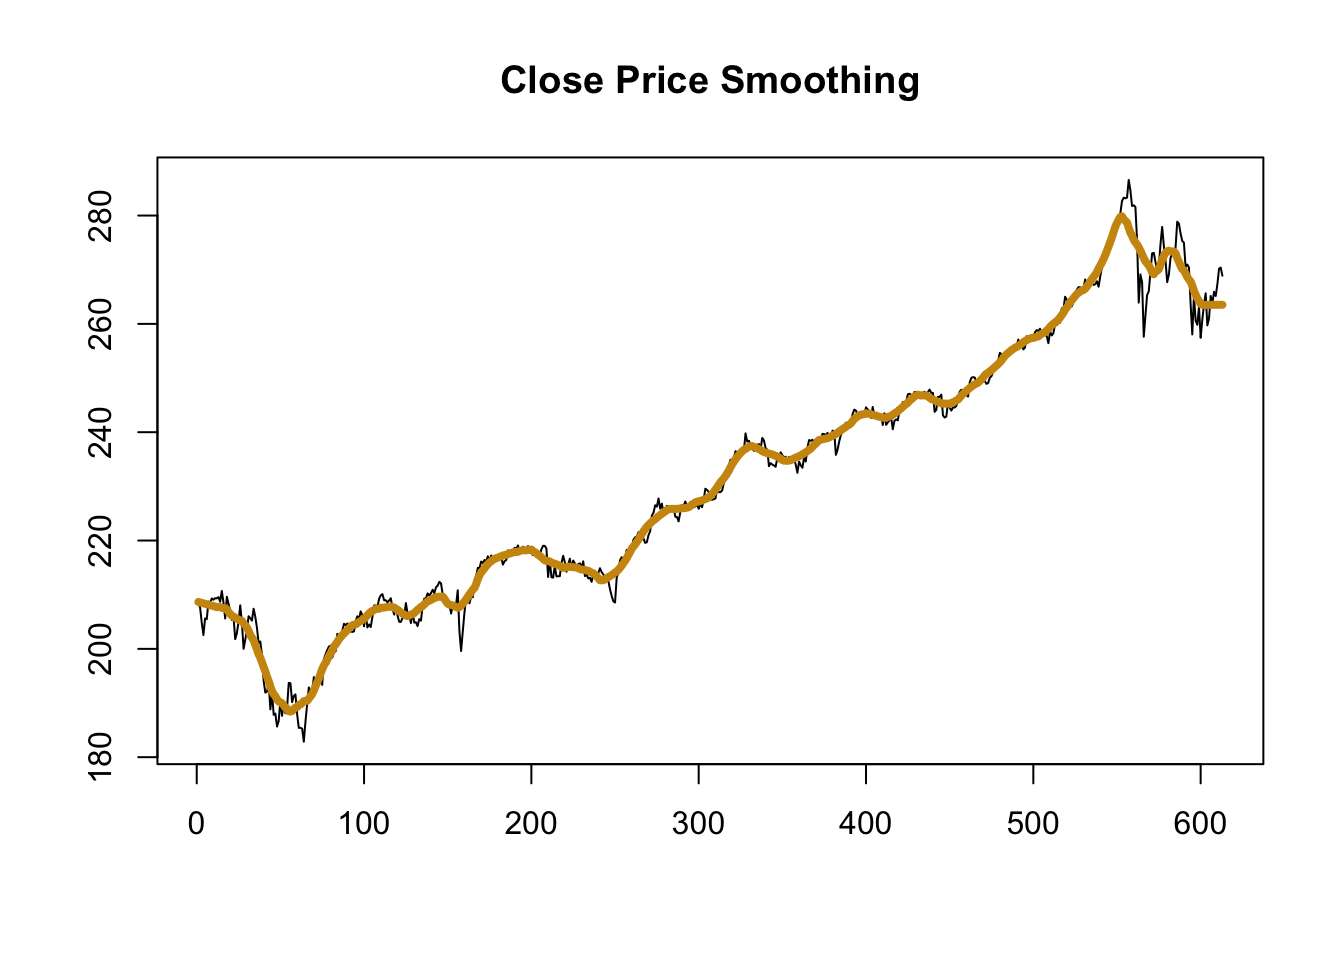
\includegraphics{SP_timeseries_files/figure-latex/unnamed-chunk-19-1.pdf}

\begin{itemize}
\tightlist
\item
  Univariate analysis
\end{itemize}

\begin{verbatim}
## `stat_bin()` using `bins = 30`. Pick better value with `binwidth`.
\end{verbatim}

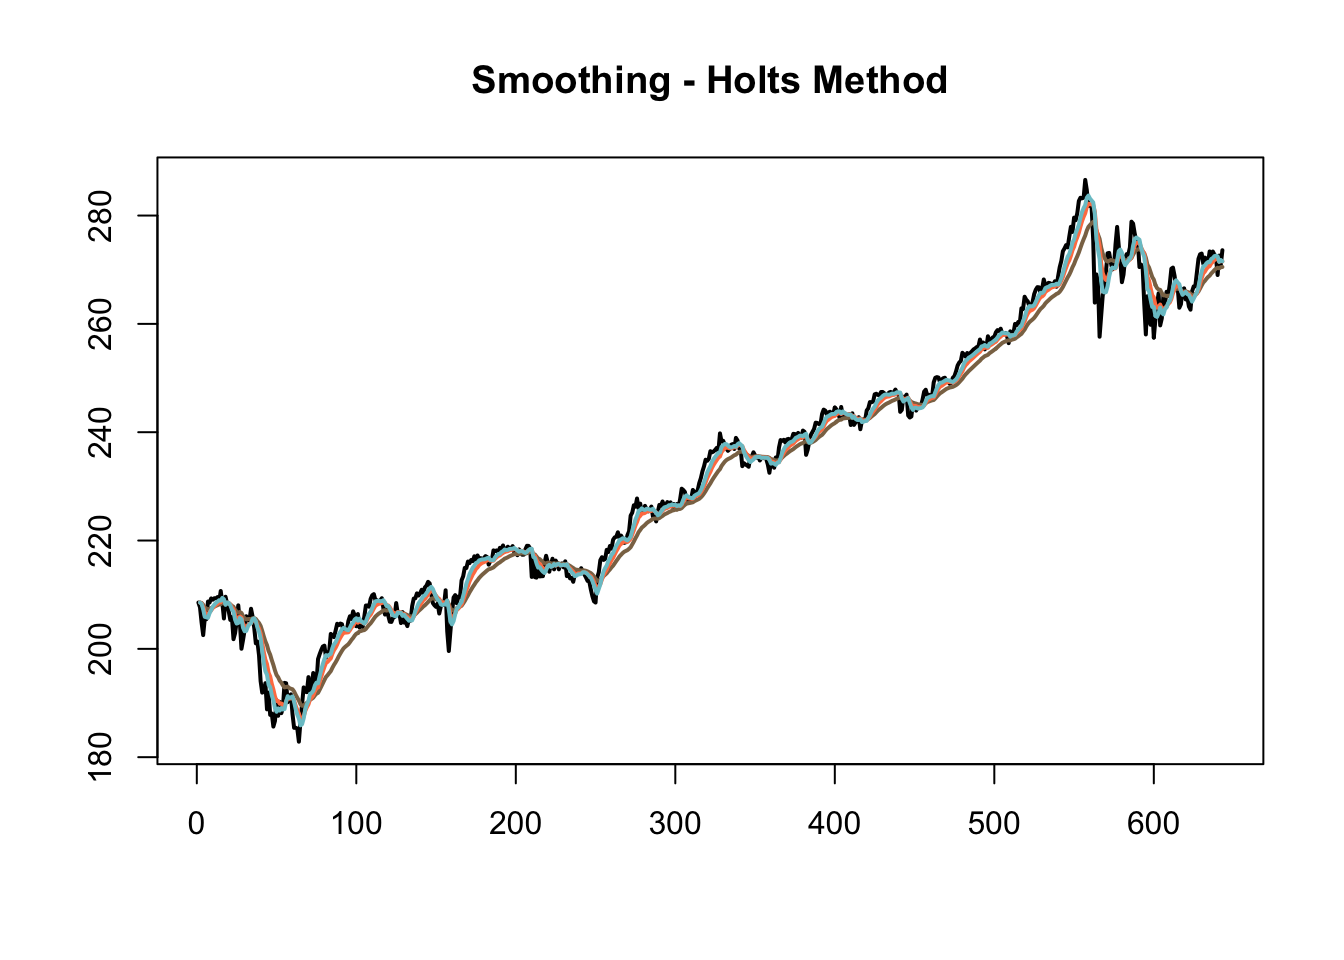
\includegraphics{SP_timeseries_files/figure-latex/unnamed-chunk-20-1.pdf}
\emph{Comments}: Most of the Pricing data is concentrated around 200 -
240

\paragraph{\texorpdfstring{Time Series Object: Creating a time series
object of
``sp\_historical\_cleaned''}{Time Series Object: Creating a time series object of sp\_historical\_cleaned}}\label{time-series-object-creating-a-time-series-object-of-sp_historical_cleaned}

\begin{verbatim}
##              open    low   high close_price    volume lead_1 lead_5
## 2015-11-10 207.51 207.19 208.60      208.55  71844000 207.67 205.47
## 2015-11-11 208.88 207.66 208.94      207.67  67251000 204.84 208.73
## 2015-11-12 206.50 204.82 207.06      204.84 118209400 202.54 208.55
## 2015-11-13 204.35 202.44 204.67      202.54 145494400 205.62 209.31
## 2015-11-16 202.32 202.18 205.69      205.62 112996000 205.47 209.07
## 2015-11-17 205.99 204.88 207.04      205.47 113429400 208.73 209.35
##            lead_10
## 2015-11-10  209.35
## 2015-11-11  209.32
## 2015-11-12  209.56
## 2015-11-13  208.69
## 2015-11-16  210.68
## 2015-11-17  208.53
\end{verbatim}

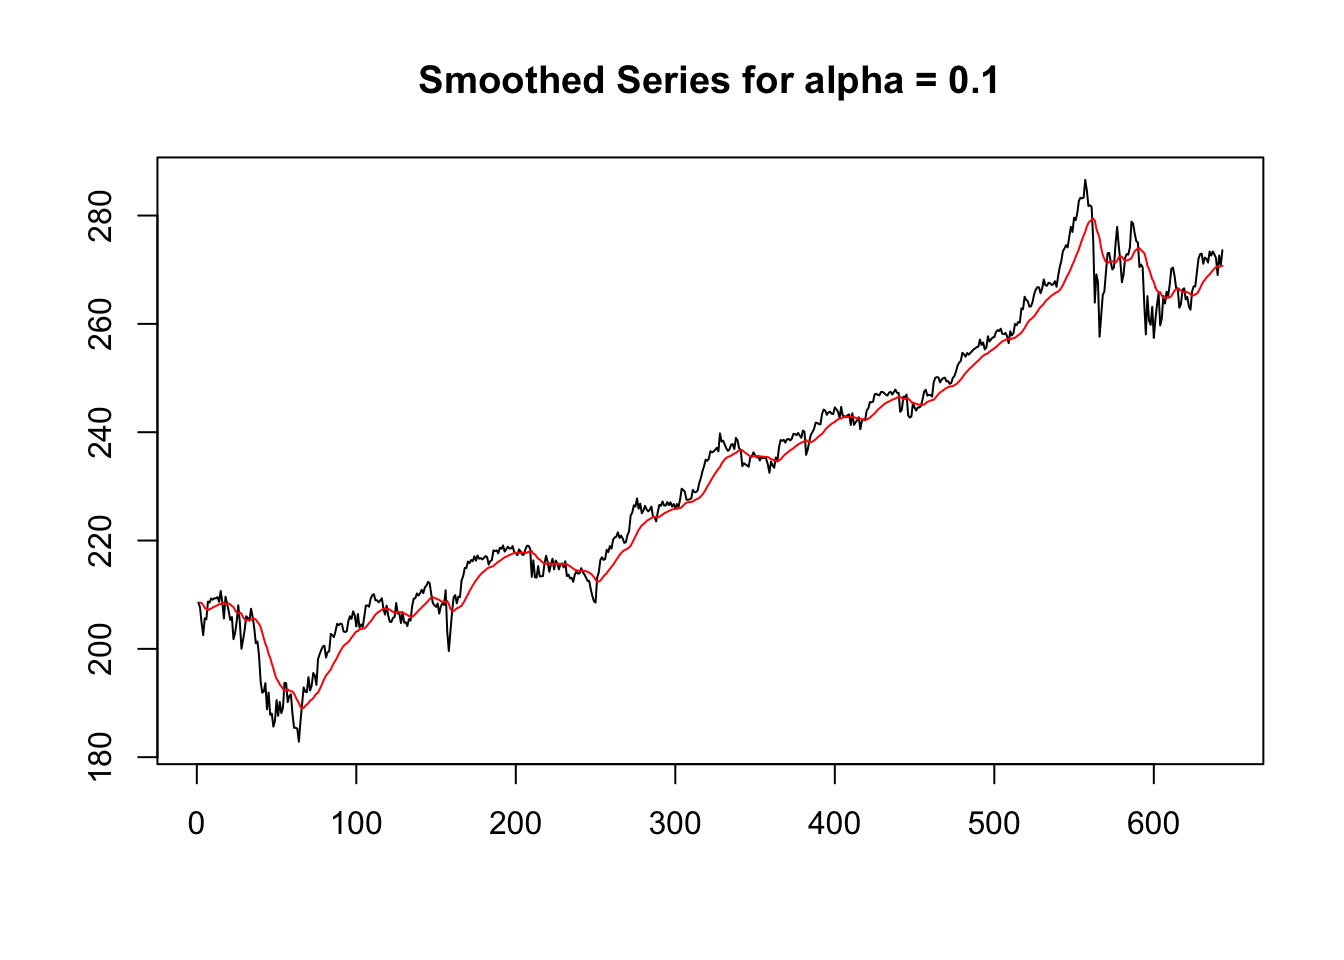
\includegraphics{SP_timeseries_files/figure-latex/unnamed-chunk-22-1.pdf}

\paragraph{Training and Validation
datasets}\label{training-and-validation-datasets}

\begin{verbatim}
##       date_txn   open    low   high close_price    volume lead_1 lead_5
## 598 2018-03-28 260.75 258.58 262.64      259.83 146088900 263.15 265.64
## 599 2018-03-29 261.12 259.84 265.26      263.15 123162700 257.47 259.72
## 600 2018-04-02 262.55 254.67 263.13      257.47 184710400 260.77 261.00
## 601 2018-04-03 258.87 256.84 261.31      260.77 119492300 263.56 265.15
## 602 2018-04-04 256.75 256.60 264.36      263.56 123193700 265.64 263.76
## 603 2018-04-05 265.55 264.32 266.64      265.64  80980400 259.72 265.93
##     lead_10
## 598  265.93
## 599  265.15
## 600  267.33
## 601  270.19
## 602  270.39
## 603  268.89
\end{verbatim}

\begin{verbatim}
##       date_txn   open    low   high close_price    volume lead_1 lead_5
## 604 2018-04-06 263.42 258.00 265.11      259.72 182029210 261.00 265.15
## 605 2018-04-09 261.37 259.94 264.84      261.00 104745500 265.15 267.33
## 606 2018-04-10 264.27 262.98 266.04      265.15 104375800 263.76 270.19
## 607 2018-04-11 263.47 263.39 265.64      263.76  90886300 265.93 270.39
## 608 2018-04-12 265.26 265.06 267.00      265.93  68138500 265.15 268.89
## 609 2018-04-13 267.41 264.01 267.54      265.15  84647281 267.33 266.61
##     lead_10
## 604  266.61
## 605  266.57
## 606  262.98
## 607  263.63
## 608  266.31
## 609  266.56
\end{verbatim}

\begin{verbatim}
## [1] 600   9
\end{verbatim}

\begin{verbatim}
## [1] 30  9
\end{verbatim}

\subsubsection{Smoothing}\label{smoothing}

\paragraph{Smoothing using Classical
Decomposition}\label{smoothing-using-classical-decomposition}

\begin{itemize}
\tightlist
\item
  window width
\end{itemize}

\begin{verbatim}
## [1] 9
\end{verbatim}

\begin{itemize}
\tightlist
\item
  Printing the smooted moving average:
\end{itemize}

\begin{verbatim}
## Time Series:
## Start = 1 
## End = 20 
## Frequency = 1 
##  [1]       NA       NA       NA       NA       NA       NA       NA
##  [8]       NA       NA 207.8979 207.8137 207.6911 207.7453 207.7058
## [15] 207.5626 207.5395 207.5026 207.3084 206.8195 206.4300
\end{verbatim}

\begin{itemize}
\tightlist
\item
  Replacing the induced NAs as result of smoothing
\end{itemize}

\begin{verbatim}
## [1] -0.08421053
\end{verbatim}

\begin{verbatim}
## [1] 0.2178947
\end{verbatim}

\begin{itemize}
\tightlist
\item
  Replacing the lagging NAs are a result of windowing of moving average
\end{itemize}

\begin{verbatim}
## Time Series:
## Start = 1 
## End = 20 
## Frequency = 1 
##  [1] 208.6558 208.5716 208.4874 208.4032 208.3189 208.2347 208.1505
##  [8] 208.0663 207.9821 207.8979 207.8137 207.6911 207.7453 207.7058
## [15] 207.5626 207.5395 207.5026 207.3084 206.8195 206.4300
\end{verbatim}

\begin{itemize}
\tightlist
\item
  Replacing the smoothed leading NAs
\end{itemize}

\begin{verbatim}
## Time Series:
## Start = 581 
## End = 600 
## Frequency = 1 
##  [1] 272.9321 272.4353 271.7326 271.4726 270.9568 270.1737 269.3974
##  [8] 268.5047 267.9321 268.1500 268.3679 268.5858 268.8037 269.0216
## [15] 269.2395 269.4574 269.6753 269.8932 270.1111 270.3289
\end{verbatim}

\begin{itemize}
\tightlist
\item
  Plotting the Smoothed Close Price
  \includegraphics{SP_timeseries_files/figure-latex/unnamed-chunk-29-1.pdf}
\end{itemize}

\paragraph{Smoothing using Holts
method}\label{smoothing-using-holts-method}

\includegraphics{SP_timeseries_files/figure-latex/unnamed-chunk-30-1.pdf}
\emph{Comments}: Clearly, from Holts Method best smoothing happens when
alpha is \textasciitilde{} 0.1

\begin{itemize}
\tightlist
\item
  Holts smoothed series Plot
\end{itemize}

\includegraphics{SP_timeseries_files/figure-latex/unnamed-chunk-32-1.pdf}

\begin{itemize}
\tightlist
\item
  Creating a new dat frame for close\_price and dates
\end{itemize}

\begin{verbatim}
##   months_smoothed smoothed_close_price
## 1               1             208.6558
## 2               2             208.5716
## 3               3             208.4874
## 4               4             208.4032
## 5               5             208.3189
## 6               6             208.2347
\end{verbatim}

\subsubsection{Model Building}\label{model-building}

\begin{verbatim}
## 
## Call:
## lm(formula = smoothed_close_price ~ cos(0.05 * months_smoothed) * 
##     poly(months_smoothed, 1) + sin(0.05 * months_smoothed) * 
##     poly(months_smoothed, 1), data = smoothed_df)
## 
## Residuals:
##      Min       1Q   Median       3Q      Max 
## -10.3422  -4.0300  -0.1904   3.7777  12.2405 
## 
## Coefficients:
##                                                       Estimate Std. Error
## (Intercept)                                          230.23069    0.19667
## cos(0.05 * months_smoothed)                           -0.02158    0.27776
## poly(months_smoothed, 1)                             567.96883    4.87636
## sin(0.05 * months_smoothed)                            1.85678    0.27629
## cos(0.05 * months_smoothed):poly(months_smoothed, 1) -88.38120    6.92574
## poly(months_smoothed, 1):sin(0.05 * months_smoothed)   6.63155    6.78174
##                                                       t value Pr(>|t|)    
## (Intercept)                                          1170.650  < 2e-16 ***
## cos(0.05 * months_smoothed)                            -0.078    0.938    
## poly(months_smoothed, 1)                              116.474  < 2e-16 ***
## sin(0.05 * months_smoothed)                             6.720 4.25e-11 ***
## cos(0.05 * months_smoothed):poly(months_smoothed, 1)  -12.761  < 2e-16 ***
## poly(months_smoothed, 1):sin(0.05 * months_smoothed)    0.978    0.329    
## ---
## Signif. codes:  0 '***' 0.001 '**' 0.01 '*' 0.05 '.' 0.1 ' ' 1
## 
## Residual standard error: 4.77 on 594 degrees of freedom
## Multiple R-squared:  0.961,  Adjusted R-squared:  0.9606 
## F-statistic:  2925 on 5 and 594 DF,  p-value: < 2.2e-16
\end{verbatim}

\includegraphics{SP_timeseries_files/figure-latex/unnamed-chunk-34-1.pdf}
\emph{Comments}: With adjusted R-Squared with accuracy of 96.2\% is the
best fit curve and it has also generated the least MAPE error of 1\%.

\begin{itemize}
\tightlist
\item
  Stationarity tests on the residual time series:
\end{itemize}

\begin{verbatim}
##         1         2         3         4         5         6 
## 12.134755 11.095516  8.121673  5.693146  8.659823  8.411551
\end{verbatim}

\begin{itemize}
\tightlist
\item
  adf test and kpss test for stationarity:
\end{itemize}

\begin{verbatim}
## Warning in adf.test(x = resi_close_price, alternative = "stationary"): p-
## value smaller than printed p-value
\end{verbatim}

\begin{verbatim}
## 
##  Augmented Dickey-Fuller Test
## 
## data:  resi_close_price
## Dickey-Fuller = -4.0685, Lag order = 8, p-value = 0.01
## alternative hypothesis: stationary
\end{verbatim}

\begin{verbatim}
## 
##  KPSS Test for Level Stationarity
## 
## data:  resi_close_price
## KPSS Level = 0.6319, Truncation lag parameter = 5, p-value =
## 0.01974
\end{verbatim}

\emph{Comments}: From these tests it can be inferred that there is
enough evidence to prove that the ``resi\_close\_price''" is Stationary.

\begin{itemize}
\tightlist
\item
  ACF and PACF Plots are:
\end{itemize}

\includegraphics{SP_timeseries_files/figure-latex/unnamed-chunk-37-1.pdf}
\includegraphics{SP_timeseries_files/figure-latex/unnamed-chunk-37-2.pdf}

\begin{verbatim}
## Series: resi_close_price 
## ARIMA(0,0,0) with non-zero mean 
## 
## Coefficients:
##          mean
##       -0.0961
## s.e.   0.2227
## 
## sigma^2 estimated as 29.81:  log likelihood=-1869.27
## AIC=3742.55   AICc=3742.57   BIC=3751.34
\end{verbatim}

\emph{Comments}: This has a very small sigma square, with a very high
log likelihood. In addition to this this is AR(0) and MA(0) time series

\begin{itemize}
\tightlist
\item
  checking the noise and stationarity of the time series using the
  box-Ljung test
\end{itemize}

\begin{verbatim}
## 
##  Box-Ljung test
## 
## data:  resi_close_price
## X-squared = 535.84, df = 1, p-value < 2.2e-16
\end{verbatim}

\emph{Comments}: thus the p-value of the time-series is very low making
it a good fit to call it a Strictly Stationary time series.

\begin{itemize}
\tightlist
\item
  QQPlot of the residual timeseries
\end{itemize}

\includegraphics{SP_timeseries_files/figure-latex/unnamed-chunk-39-1.pdf}
\emph{Comments}: QQ plot suggests that Close\_price time-series is
stationary

\begin{itemize}
\tightlist
\item
  Plotting the histogram of the residual time-series represents a
  Gaussian Curve
\end{itemize}

\includegraphics{SP_timeseries_files/figure-latex/unnamed-chunk-40-1.pdf}

\begin{itemize}
\tightlist
\item
  Checking the properities of Residual time-series by inspection
\end{itemize}

\includegraphics{SP_timeseries_files/figure-latex/unnamed-chunk-41-1.pdf}
\emph{Comments}: Thus, it is also clear from the plots ARIMA, ADF test,
KPSS test the that the time series is stationary

\subsubsection{Model Evaluation}\label{model-evaluation}

\begin{itemize}
\tightlist
\item
  Predicting the values fitted model from the vadlidation dataset
\end{itemize}

\begin{verbatim}
##   months_smoothed
## 1             601
## 2             602
## 3             603
## 4             604
## 5             605
## 6             606
\end{verbatim}

\begin{itemize}
\tightlist
\item
  MAPE Error - Accuracy Calculation
\end{itemize}

\begin{verbatim}
## [1] 1.026822
\end{verbatim}

\emph{Comments}: Thus with a MAPE error of just 1.0268, model is
apparently a very good fit.

\begin{itemize}
\item
  Combining the predicted values train and test data
\item
  Plottig the actual vs the predicted data, using classical
  decomposition
\end{itemize}

\includegraphics{SP_timeseries_files/figure-latex/unnamed-chunk-45-1.pdf}

\subsubsection{PREDICTION ANALYSIS USING
AUTO.ARIMA}\label{prediction-analysis-using-auto.arima}

\paragraph{Modelling auto arima}\label{modelling-auto-arima}

\begin{verbatim}
## Series: sp_train$close_price 
## ARIMA(4,1,0) 
## 
## Coefficients:
##           ar1      ar2     ar3     ar4
##       -0.0655  -0.0858  0.0847  0.0362
## s.e.   0.0409   0.0410  0.0411  0.0416
## 
## sigma^2 estimated as 3.148:  log likelihood=-1191.36
## AIC=2392.73   AICc=2392.83   BIC=2414.7
## 
## Training set error measures:
##                      ME     RMSE      MAE        MPE      MAPE     MASE
## Training set 0.09879535 1.766713 1.188871 0.03878482 0.5244785 0.999416
##                      ACF1
## Training set -0.002495871
\end{verbatim}

\begin{itemize}
\tightlist
\item
  Predicting the Validation dataset
\end{itemize}

\includegraphics{SP_timeseries_files/figure-latex/unnamed-chunk-47-1.pdf}

\begin{itemize}
\tightlist
\item
  MAPE of Close Price Using Auto Arima.
\end{itemize}

\begin{verbatim}
## [1] 1.079454
\end{verbatim}

\begin{itemize}
\item
  Combining the predicted training and testing to plot
\item
  Combined plot of Arima
\end{itemize}

\includegraphics{SP_timeseries_files/figure-latex/unnamed-chunk-50-1.pdf}

\subsubsection{Conclusion}\label{conclusion}

\begin{itemize}
\tightlist
\item
  Thus the Accuracy result using the MAPE using Classicial Decomposition
  is 1.03 which is less than Auto.Arima Modelling 1.08 and Classical
  Decompsition has had higher accuracy*
\end{itemize}


\end{document}
